\subsection{PLR-based Approximate Indexing}
\label{sec:design:plr-basic}

To further reduce the memory usage, \ours{} takes a more aggressive approach
using PLR which has a potential to
express many entries <$x_i$, $y_i$> using a few linear equations. 

Given $R_i$ = \{<$x_0$, $y_0$>, <$x_1$, $y_1$>, ..., <$x_{n-1}$, $y_{n-1}$>\},
\ours{} transforms $R_i$ into a set of line segments 
$R_i^{PLR}$ = \{$S_0$, $S_1$, ..., $S_{k-1}$\} using PLR.
Each line segment $S_h$ is modeled by a linear equation, $y_i'=a_h(x_i-x_h)+b_h+y_h$, 
where $a_h$ is a slope, $b_h$ is an intercept, and $x_h$ and $y_h$ are
the first x-y coordinate of $S_h$ in the run.
It approximates the physical location $y_i$ of $x_i$.
A predicted location $y_i'$ is within a bounded error $\delta$.
That is, $y_i'$ is guaranteed to lie within [\PSA{i} - $\delta$, \PSA{i} + $\delta$).

\begin{figure}[t]
\centering
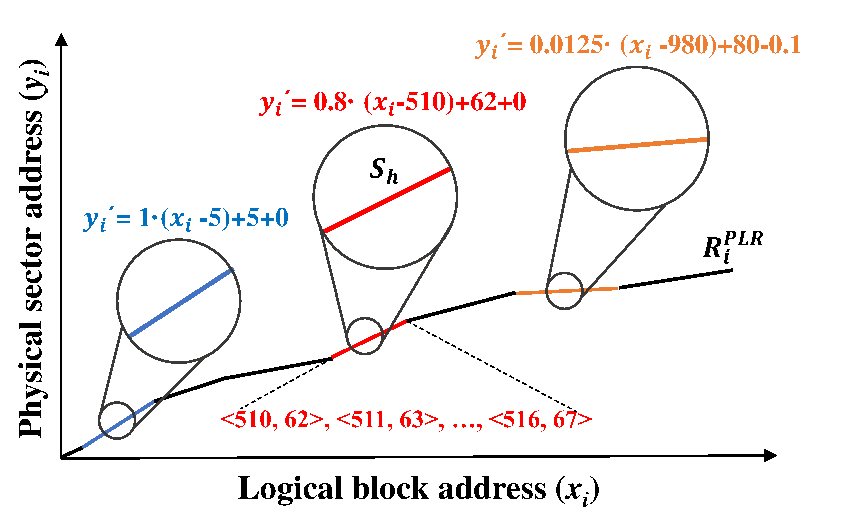
\includegraphics[width=0.34\textwidth]{figs/OSDI/PLR_org.eps}

\caption{Examples of PLR-based approximate indexing}
\label{fig:plr_base}
\vspace{-5pt}
\end{figure}

Similar to the FP-based indexing, \ours{} creates a PLR-indexed table for a new run
that is being created during compaction, and its copy is stored in the flash as
part of the run's metadata.  A PLR table keeps parameters of linear
equations: $a_h$, $b_h$, $x_h$, and $y_h$ for $S_{h}$.
\FIG{fig:plr_base} shows the example of how \ours{} converts $R_i$ = \{...,
<510, 62>, <511, 63>, ..., <516, 67>, ...\} into $R_i^{PLR}$ = \{..., $S_h$,
...\}, where $S_h$ is expressed as the linear equation
$y_i'=0.8\cdot(x_i-510)+62$.

To retrieve data for \LBA{i}, \ours{} finds a designated run using the shortcut table
and then performs binary search to find a PLR model by looking up x-coordinates
in a PLR table. Taking the example of \FIG{fig:overall:plr} where \LBA{i} =
515 comes to query, the model returns $y_i'=66$ and $\delta$ is 0 since $y_i=66$. 
\ours{} also suffers from a prediction error. If $x_j=513$, the predicted
$y_j'=64.4$ with $\delta$ of 0.6.  To resolve an error, extra I/Os are
unavoidable.  In the following subsection, we explain how \ours{} controls an
error rate $\mathcal{E}_{PLR}$ of the PLR-based indexing and applies it to PLR
models.
%This may lead to extra I/Os to resolve an error.
%Similar to the FP-based indexing, we design the PLR-based indexing
%so that it guarantees a target error rate, trading 
%DRAM usage.  
%Looking up and building PLR models should be performed
%efficiently as well.  

%To achieve the above goals, we refactor the original PLR
%algorithm (OptimalPLR~\cite{plr3}) that has a general-purpose design for any
%applications. By refactoring it suitable for \ours{}, we can express a linear
%equation using fewer bits without sacrificing prediction accuracy too much.  We
%also minimize user-perceived performance penalties by building PLR models while
%performing compaction I/Os.  A detailed explanation is given in
%\SEC{sec:design:plr}.
\begin{figure}[b]
\centering
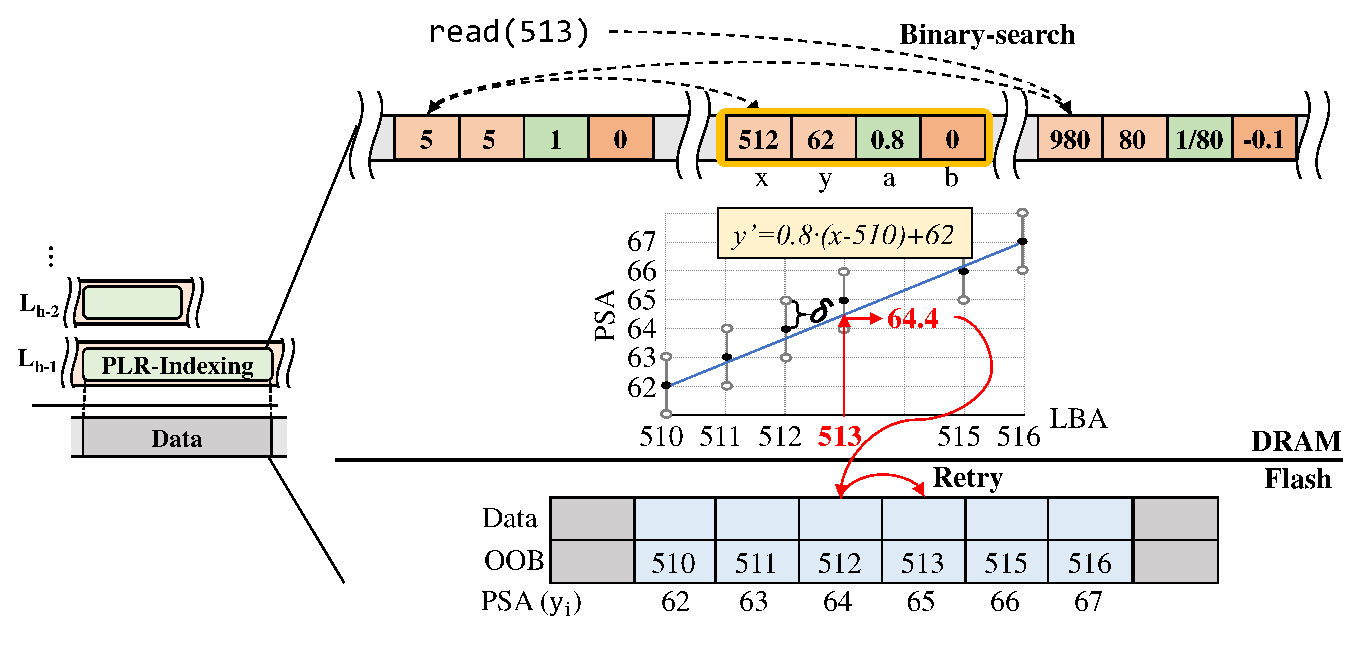
\includegraphics[width=0.45\textwidth]{figs/OSDI/PLR.eps}
\vspace{-5pt}
\caption{PLR-based approximate indexing and its operations}

\label{fig:overall:plr}
\end{figure}

\subsubsection{PLR Error Rate Control}
\begin{figure}[t]
\centering
%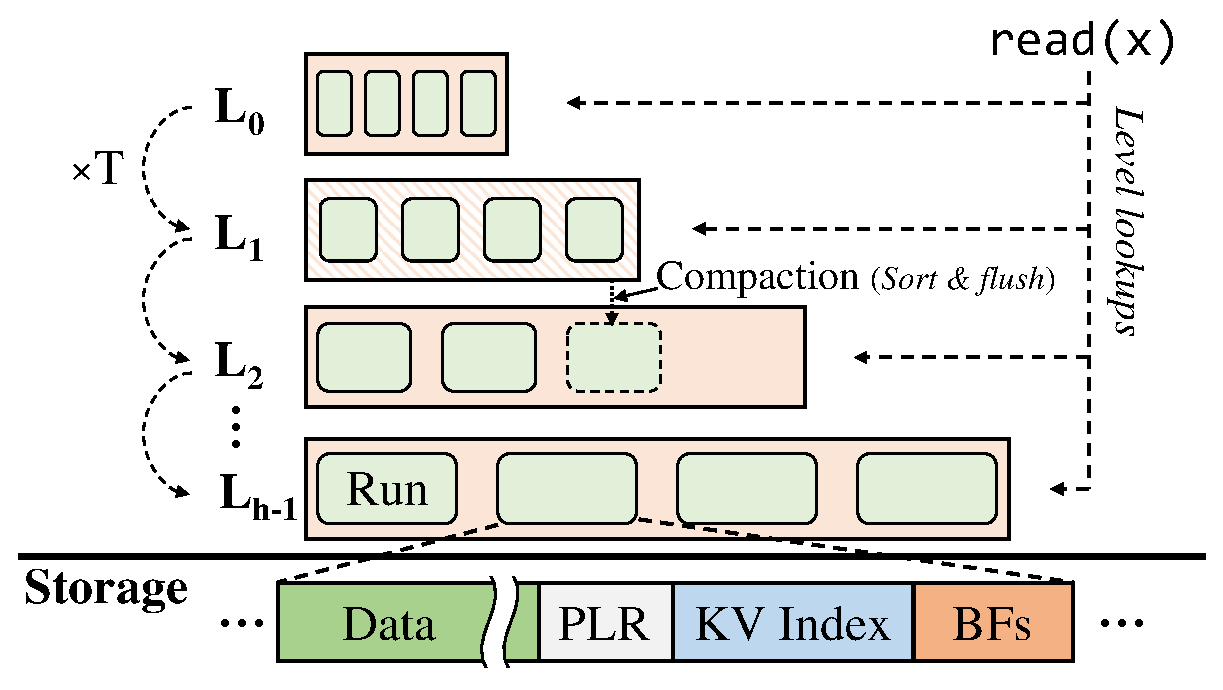
\includegraphics[height=3.3cm]{fig2.eps}
\includegraphics[height=2.5cm]{figs/OSDI/plr-ctr.eps}
\caption{Error control in PLR}
\label{fig:plr-control}
\vspace{-5pt}
\end{figure}

Let us first take a look at the
organization of NAND flash in \FIG{fig:plr-control}, where 
4KB logical blocks, $x_{i}$, $x_{i+1}$, $x_{i+2}$, and $x_{i+3}$
are stored in four consecutive 4KB sectors, $y_{i}$,
$y_{i+1}$, $y_{i+2}$, and $y_{i+3}$.
The four sectors belong to the same NAND page.
Since a page is the unit of I/O in the flash, the logical blocks (or physical sectors) are
read together. 

In \FIG{fig:plr-control}, assuming that $\delta$ is set to 1.5 when building the
PLR model, so that the error of the predicted $y_i'$ is less than 1.5.
Under a fully random workload, when serving a read request to $x_{i}$, the
probability of requiring more than one page read is 33\%
(\ie~$\mathcal{E}_{PLR}$ of 0.33).  If $-0.5 \leq y_i'-y_i < 1.5$, one 16KB page
read is sufficient to service $x_{i}$ without any trial errors.  Only when
$-1.5 \leq y_i'-y_i < -0.5$, a neighboring page is read unnecessarily.  For
$x_{i+1}$, $x_{i+2}$, and $x_{i+3}$, their $\mathcal{E}_{PLR}$s are estimated as
0, 0, and 0.33, respectively. As a result, the average $\mathcal{E}_{PLR}$
is 0.167 when $\delta$ is 1.5.

By reducing $\delta$, we can make $\mathcal{E}_{PLR}$ smaller.  If
$\delta = 0.83$, $\mathcal{E}_{PLR}$ of 0.1 is ensured.  However, setting
$\delta$ so tightly ($\delta$ = 0.1) comes at the cost of more memory
usage.  This is because the PLR algorithm has to create more line
segments in $R_{PLR}$, so as not to violate a narrow range of $\delta$.  
If $\delta$ is too large (\eg~$\delta = 10$), 
PLR creates $R_i^{PLR}$ with fewer segments but suffers from many errors. 
Developing a new PLR
algorithm that creates a smaller number of line segments with tight $\delta$
is beyond our scope.  Instead, we aim to reduce memory
requirement of line segments through system-level optimizations.

%because each line segment is able to cover many
%mapping pairs without violation of the designated $\delta$. 

%We may further reduce extra I/Os caused by errors by 

%Reducing $\delta$ further may lower extra I/Os caused by errors.  However, this
%comes at the cost of more memory.  Given the same input $R_i$.  the PLR
%algorithm needs to create more line segments if $\delta$ is set so tightly.
%Conversely, if $\delta$ is too large (\eg~$\delta=0.5$), the PLR creates
%$R_i^{PLR}$ with fewer segments because each line segment is able to cover many
%mapping pairs without violation of the designated $\delta$. \FIG{todo} displays
%the number of line segments needed to cover the same $R_i$ depending on
%$\delta$.
    

\begin{comment}
\begin{figure}[t]
\centering
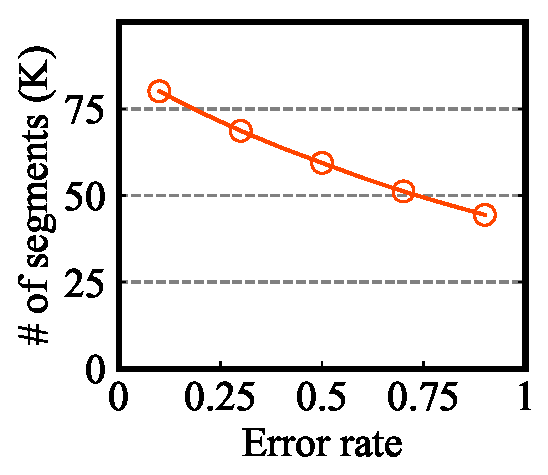
\includegraphics[height=3cm]{figs/OSDI/PLR-Error.eps}
\vspace{-10pt}
\caption{\FIXME{Number of line segments under varying error rates}}
\vspace{-10pt}
\label{fig:plr-error-memory}
\end{figure}

{
\renewcommand{\arraystretch}{0.4}
\begin{table}[t]
    \small
    \caption{Bits-per-line-segment (BPL) after PLR optimization}
    \vspace{-10pt}
    \centering
    \begin{tabular}{|c||c|c|c|c|}
        \hline
                                 &  {Unoptimized}  & {+Slope}  & {+Intercept}  & {+Delta}  \\
                                & {PLR} & {quantization} & {quantization} & {encoding}\\\hline
    BPL	    &  256-bit     &    203-bit     & 151-bit      &46.2-bit   \\ \hline
    \end{tabular}
    \label{tab:plr-opt}
    \vspace{-10pt}
\end{table}
}
\end{comment}

\subsubsection{Memory Optimization}

The PLR itself is memory efficient, but there exists room to further
improve its memory efficiency.  
To model a various range of $<x_i, y_i>$ pairs supplied as an input,
the original PLR uses real numbers, 8B each, for four components of a linear equation. 
Each line segment thus needs 32B in total, which dwarfs its
memory efficiency.  
%The original PLR provides higher
%memory efficiency than exact indexing, but cannot outperform the BF-based
%indexing (see \FIG{fig:tree-org}(a) in \SEC{sec:design:tree}).
%Fortunately, unlike typical use cases of PLR where 
%a various range of $<x_i, y_i>$ pairs are provided as an input,
\ours{} has quite regular $<x_i, y_i>$ patterns within each run,
thanks to the property of an LSM-tree.
%thanks to the sorted nature of the LSM-tree.
%In \ours{}, $x_i$ increases monotonically all the time 
%(\ie~$x_i < x_j$ if $i < j$) because of sorted nature of the LSM-tree.
%Moreover, $y_i$ always increases by 1 since all the incoming data
%is appended to the run.
By leveraging such properties, \ours{} applies (\textit{i}) quantization and
(\textit{ii}) delta-encoding to reduce the sizes of four line parameters,
$a_h$, $b_h$, $x_h$, and $y_h$.
%It enables us to construct memory-efficient PLR models without sacrificing
%accuracy too much.
%Table~\ref{tab:plr-opt} summarizes
%the number of bits per line segment after applying
%optimization techniques to the PLR-based indexing.
%through quantizing and compressing the components.
%\ours{} leverages such properties to construct memory-efficient models.
%\todo{(최적화 기법들에 대한 간단한 언급???)}




\begin{comment}
\begin{figure}[t]
    \centering
    \begin{subfigure}[b]{0.17\textwidth}
         \centering
         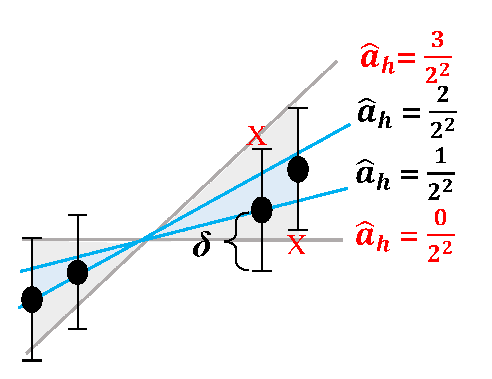
\includegraphics[width=\textwidth]{figs/OSDI/slope_quant.eps}
         \vspace{-10pt}
         \caption{Slope quantization}
         \vspace{-10pt}
    \end{subfigure}
    \hfill
     \begin{subfigure}[b]{0.15\textwidth}
         \centering
         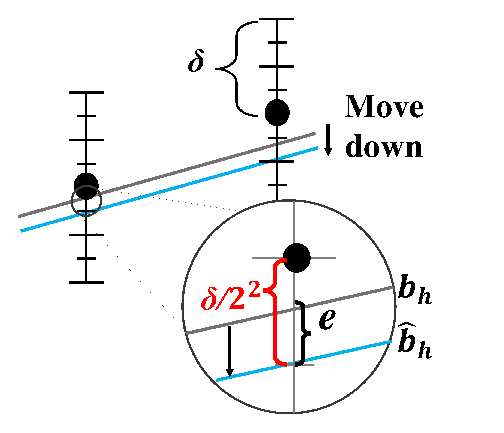
\includegraphics[width=\textwidth]{figs/OSDI/inter-quant.eps}
         \vspace{-10pt}
         \caption{Intercept quantization}
         \vspace{-10pt}
    \end{subfigure}
    \caption{Slope and intercept quantization ($t=2$)}
\label{fig:plr_opt}	 
\end{figure}
\end{comment}
\textbf{Slope Quantization.} 
Typical PLR algorithms consider a broad range of possible slopes $\rho$
($-\infty<\rho<\infty$) to create a smaller
number of line segments.  \ours{} can
create almost the same number of line segments as that of typical PLRs even if a range of $\rho$ is
limited to $0 < \rho \leq 1$ because of the following two properties.

First, the highest slope of the line segment that \ours{} has is at most 1.0.
This extreme case occurs where both $x_i$ and $y_i$ increase
monotonically by 1, for example, $R_i$ = \{<5, 5>, <6, 6>, ...,
<20, 20>\} (see the first segment in \FIG{fig:plr_base}). Second, the lowest
slope in \ours{} is at least higher than 0.0. This happens when $x_i$ increases
much faster than $y_i$, for example, $R_i$ = \{<980, 80>, <1060, 81>, <1139,82>,
..., <3380, 110>\} (see the third segment in \FIG{fig:plr_base}).
%Therefore, even if \ours{} models a given $<x_i, y_i>$ pairs with
%possible slope $0 \leq \rho \leq 1$, it can find a sufficiently small number of
%line segments.

This narrow slope range makes it easier that $a_h$ is expressed by
fewer bits.  \ours{} uses only $t$-bit to express $a_h$ by
quantizing a slope range into $2^t$
discrete finite ones ($\frac{0}{2^t}$, $\frac{1}{2^t}$, ...,
$\frac{2^t-1}{2^t}$) as shown in \FIG{fig:plr_opt}(a). 
The quantized version $\hat a_h$ of $a_h$
is defined as $\hat a_h = \Delta \cdot \floor*{\frac{a_h}{\Delta}}$, 
where the step size $\Delta$ is $\frac{1}{2^t}$.
Owing to quantization errors,
we may not create a line segment even if there exist possible
slopes expressed by an 8B real number.
%Consider $t=2$ where $\hat a_{(i,j)}$ can express 0.0, 0.25,
%0.5, and 0.75 slopes.  
%Suppose $t=2$ and $\hat a_{(i,j)}$ can be 0.0, 0.25,
%0.5, or 0.75. If a feasible slope range $\rho$ lies between 0.6 and 
%0.7, no line segments can be created. 
This results in more
line segments, which in turn leads to memory waste.  
But, when $t$ = 11, the number of line
segments generated is similar to that of 
OptimalPLR~\cite{plr3}, an optimal PLR algorithm generating
the minimal number of segments.

\begin{figure}[t]
\centering
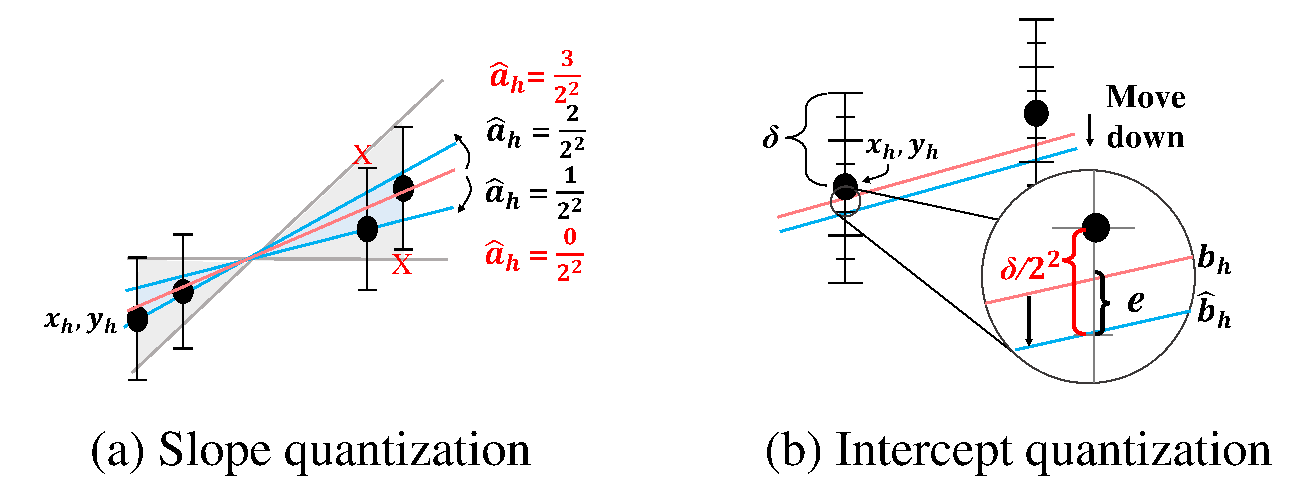
\includegraphics[width=0.43\textwidth]{figs/OSDI/PLR_opt_2.eps}
\caption{Slope and intercept quantization ($t=2$)}
\label{fig:plr_opt}
\end{figure}

\textbf{Intercept Quantization.}
Since the number of possible slopes is limited to $2^t$, possible intercepts
$b_h$ on the y-axis are also limited.  To take advantage of this
property, we quantize $b_h$, expressing it using a finite discrete
number. 
For any feasible line segment, $b_h$ must be in the range $-\delta\leq
b_h\leq\delta$. \ours{} uniformly divides the possible range $2 \cdot
\delta$ of $b_h$ into $2^{t+1}$ quantized levels with the step size
$\Delta = \frac{\delta}{2^t}$.  Thus, only $t+1$-bit is needed to represent a
quantized intercept.  The quantized version $\hat b_h$ of $b_h$
is expressed as $\hat b_h = \Delta \cdot \floor*{\frac{b_h}{\Delta}}$.  

With the intercept quantization, the original line segment
vertically moves down (see \FIG{fig:plr_opt}(b)) 
since the floor function is used to quantize $b_h$.
Owing to the error, the quantized line segment may violate the condition 
$|y'_i-y_i|\leq\delta$.
This also results in more line segments, wasting memory.
Currently, we use the same $t=11$ for the intercept
quantization which is large enough. The violation rarely happens in
practice.  

\textbf{Delta-encoding.}
To express the first x-y coordinate $x_h$ and $y_h$ of $S_h$,
\ours{} uses two 4B integers.
To further reduce their sizes, \ours{} employs delta-encoding.  
Given two consecutive
line segments $S_h$ and $S_{h+1}$, \ours{} only keeps 
deltas $x_{h+1} - x_{h}$ and $y_{h+1} - y_h$ for $S_{h+1}$, instead of
$x_{h+1}$ and $y_{h+1}$.
The delta-encoding effectively saves memory requirement.
However, to find a line segment that contains a specific $x_i$, we have
to scan the PLR-indexed table while performing delta-decoding.  
To mitigate the overhead, we take the similar approach used in the FP-indexed table.
\ours{} splits the PLR-indexed table into multiple PLR groups
and maintains uncompressed $x_h$ and $y_h$ at the beginning of each group.
%for every $d$ fragment, \ours{} maintains a pivot pair that keeps uncompressed
%$x_i$ and $y_i$.  
In this way, 
\ours{} can quickly find a wanted PLR group via binary-search 
and retrieve a desired line segment by scanning a smaller number of candidates.
The time complexity 
is $O(log_{2}\frac{f}{d}+d)$, where $f$ is the number of line segments in a run
and $d$ is the number of line segments in a group.

\subsubsection{Lookup Optimization}
To balance the lookup latency against memory consumption,
we also apply the similar optimization as we did for the FP-indexed table
when deciding the size of each PLR group.
For delta-compressed x-y coordinates,
we assign 11-bit and 9-bit, respectively.
For every PLR group, we should maintain uncompressed $x_h$ and $y_h$,
each of which requires a 4B integer (if the SSD capacity is 16TB).
Since $a_h$ and $b_h$ need 11-bit and 12-bit, respectively, 
we can pack one uncompressed segment (87-bit) and 
9 compressed segments (43-bit each), 10 segments in total,
into a 64B CPU cache line. Considering that 
the original PLR requires 256-bit per segment, \ours{} achieves 5$\times$ memory efficiency to express a line segment.


\begin{comment}
The memory space required for $m_{(i,j)}$ in a run is 
$f \cdot \{\mathcal{C}(x_i)+\mathcal{C}(y_i)\}$, where $\mathcal{C}(x_i)$ and
$\mathcal{C}(y_i)$ are the numbers of bits required for delta-encoded $x_i$
and $y_i$.  Currently,
$\mathcal{C}(x_i)$ and $\mathcal{C}(y_i)$ are 11-bit and 9-bit,
respectively.  For (uncompressed) pivot pairs, \ours{} still needs two 4B
integers, along with a 4B index that points to the start
location of compressed fragments to scan.  The memory consumption of pivot
pairs is $\frac{f}{d} \cdot (4 + 4 + 4)$\ bytes.
If $d$ is 30, for every 30 fragments, a 12B pivot pair is needed.
The memory overhead per each fragment is thus 3.2-bit.

In summary, for the four parameters of the linear equation, the original PLR
needs 256-bit ($= 64 + 64 + 64 + 64$).  
\ours{} reduces it to 46.2-bit ($= 11 + 12 + 11 + 9 +  3.2$) where $t
= 11$, $\mathcal{C}(x_i) = 11$, 
$\mathcal{C}(y_i) = 9$ and the pivot overhead per fragment is $3.2$.
If the number $f$ of fragments is the same as the two, 
we achieve 5.5$\times$ memory
efficiency over the original PLR.
\end{comment}


\begin{comment}
\subsubsection{PLR Model Creation}

We first formally explain how \ours{} creates PLR models using an example in
\FIG{fig:plr-indexing}.  Let $M = \{m_1, m_2, ..., m_n\}$ be a set of mapping
pairs $m_i = (x_i, y_i)$ in a run.  We use $m_{(i, j)} = \{m_i, m_{i+1}, ...,
m_j\}$ $(1\leq i < j \leq n)$ to denote a set fragment.  
%Given $M$ and a target error bound $\delta$, \ours{} divides $M$ into set
%fragments, so that each fragment $m_{(i, j)}$ is represented by a line segment
%whose linear function $y_h' = a \cdot x_h +b$ satisfies $|y_h' - y_h| \leq
%\delta$ for any pair $m_h = (x_h, y_h)$ in $m_{(i,j)}$.
Given $M$ and a target error bound $\delta$, \ours{} divides $M$ into set
fragments so that each fragment $m_{(i, j)}$ is modeled by a line segment
whose linear equation $y_h' = a \cdot x_h +b$ satisfies $|y_h' - y_h| \leq
\delta$ for any pair $m_h = (x_h, y_h)$ in $m_{(i,j)}$.  \ours{} maintains
multiple set fragments for $M$.  Thus, the linear equation of the line segment
for $m_{(i, j)}$ is defined as follows:
\begin{equation}
\small
\begin{split}
	y_h' = a_{(i, j)} \cdot (x_h - x_i) + y_i + b_{(i, j)},
\end{split}
\label{eq:linear}
\end{equation}
%where $x_i$ and $y_i$ are from the first pair $m_i$ and used as a base
%point where $m_{(i, j)}$ starts.  
where $x_i$ and $y_i$ are coordinates where $m_{(i, j)}$ starts.  $a_{(i, j)}$
is the slope of the line segment for $m_{(i, j)}$, and $b_{(i, j)}$ is the
relative intercept of the line from \PSA{i}.  
In \FIG{fig:plr-indexing} where seven pairs $m_1=(2,1)$, ..., $m_7=(46,7)$ are
given, there are two line segments for $m_{(1,4)}$ and $m_{(5,7)}$. $m_1=(2,1)$
and $m_5=(43,5)$ are start coordinates. For $m_{(1,4)}$, $a_{(1,4)}=0.6$ and
$b_{(1,4)}=0$, and for $m_{(5,7)}$, $a_{(5,7)}=0.33$ and $b_{(5,7)}=0.5$.


Four parameters, $a_{(i, j)}$, $b_{(i, j)}$, $x_i$, and $y_i$, are kept in
DRAM.  Thus, it is important to construct a small number of line segments 
to save memory. \ours{} uses OptimalPLR~\cite{plr3} to find an
optimally minimal number of line segments. OptimalPLR is designed 
for online streams and thus is fast.
We explain how \ours{} creates line segments using OptimalPLR below.

\begin{figure}[t]
\centering
%\includegraphics[height=5.3cm]{test.eps}
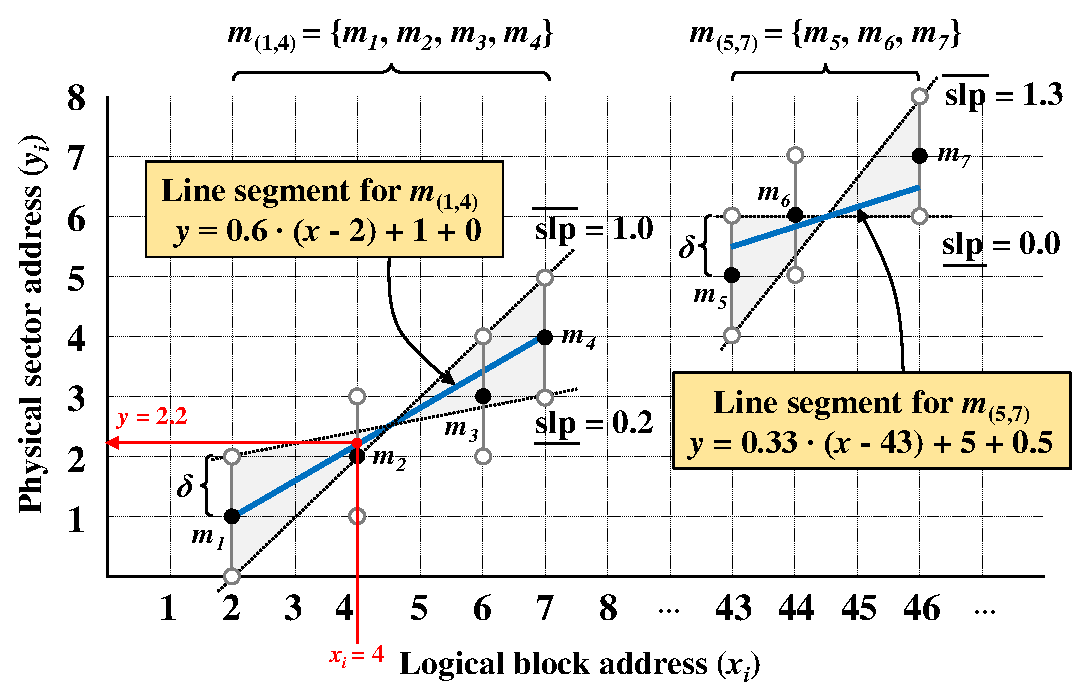
\includegraphics[height=5cm]{./figs/figs-final/fig-plr.eps}
\vspace{-10pt}
\caption{Examples of PLR-based approximate indexing}
\vspace{-10pt}
\label{fig:plr-indexing}
\end{figure}

Initially, \ours{} starts with no set fragments. Given $M$, it creates an empty set
fragment and adds a mapping pair from $M$ to the fragment one by one.
After adding a new pair (and if at least two pairs exist), 
\ours{} sees if there is a line segment that satisfies a
lower error bound than $\delta$ for all the pairs in the fragment. Let
$m_{(1,k)}$ be the fragment to be tested.  According to~\cite{plr3}, \ours{}
computes the minimum slope $\minslp{}$ and the maximum slope
$\maxslp{}$ of $m_{(1,k)}$, which are defined as follows:
\begin{equation}
\small
\begin{split}
\minslp{} &= \max_{1 \le i < j \le k}{\frac{(y_j-\delta)-(y_i+\delta)}{x_j - x_i}}. \\
\end{split}
\label{eq:min-slp}
\end{equation}
\begin{equation}
\small
\begin{split}
\maxslp{} &= \min_{1 \le i < j \le k}{\frac{(y_j+\delta)-(y_i-\delta)}{x_j - x_i}}. \\
\end{split}
\label{eq:max-slp}
\end{equation}

According to the Corollary 1 in~\cite{plr3}, if $\minslp{} \leq \maxslp{}$, there
exist feasible line segments that satisfy a lower error bound than $\delta$.
Feasible line segments pass the intersection point of the $\maxslp{}$ line and 
the $\minslp{}$ line,
and  their slopes $\rho$ are in the range $\minslp{} \leq \rho \leq
\maxslp{}$.  If $\minslp{} > \maxslp{}$, there are no feasible line segments.
If feasible line segments are found, 
\ours{} moves on to the next pair
$m_{k+1}$ by adding it to the fragment and sees if there exist feasible lines
for $m_{(1, k+1)}$.  
If no feasible lines exist (\ie~$\minslp{} > \maxslp{}$ in $m_{(1, k+1)}$), 
\ours{} closes the fragment with
pairs from $m_1$ to $m_k$.  It then chooses one of the possible $\rho$ slopes,
$a_{(1, k)}$, for $m_{(1, k)}$. The intercept $b_{(1, k)}$ is
obtained accordingly.  From $m_{k+1}$, \ours{} repeats the above steps
until it creates all the line segments to approximate
$M$.

%a feasible slope(s) $\rho$ in the range $\minslp{} \leq \rho \leq \maxslp{}$
%that creates the linear function satisfying a lower error bound than $\delta$.
%(There may exist many feasible lines).  
%If it fails to find any feasible one, 

In the example of \FIG{fig:plr-indexing}, $m_{(1,4)}$ has $\maxslp{}=1.0$ and
$\minslp{}=0.2$. Thus, there exist many feasible line segments whose slopes are
in the range $0.2 \leq \rho \leq 1.0$ (highlighted in gray).  
After adding $m_5$ to $m_{(1,4)}$, $\maxslp{}$ drops to 0.15, while $\minslp{}$
still remains 0.2. Thus, no feasible line segments exist.
$m_{(1,4)}$ becomes a fragment, and $a_{(1,4)}$ and 
$b_{(1,4)}$ are chosen to be 0.6 and 0.0. 
%\ours{} then starts with $m_5$ to create a new segment.

After creating line segments for $M$, we minimize the memory usage by
reducing the size of equation parameters.  We use quantization to reduce
a slope $a_{(i, j)}$ and an intercept $b_{(i, j)}$ and apply delta-encoding 
to independent $x_i$ and dependent $y_i$ variables.

\subsubsection{Memory Optimization}
\label{sec:plr:memory}

\textbf{Slope quantization.} 
Theoretically, $\minslp{}$ and $\maxslp{}$ can be any numbers.  PLR
algorithms thus aim to cover a broad range of slopes $\rho$ using an 8B
real number to generate an optimal number of line segments.  
Without losing optimality, by Theorem 1, \ours{} finds feasible line segments 
even if the range of $\rho$ is limited to $0 \leq \rho \leq 1$.

\textit{\textbf{Theorem 1}}  \ \textit{Suppose that for a given $m_{(i,j)}$, $\minslp{} \leq
\maxslp{}$ is satisfied and feasible line segments exist whose possible slopes $\rho$
are in the range $\minslp{} \leq \rho \leq \maxslp{}$. Even if the slope range 
is limited to $0 \leq \rho \leq 1$, feasible line segments can be found in $m_{(i,j)}$.}

\textit{\textbf{Proof}} \ 
For any pairs of $\minslp{}$ and $\maxslp{}$ that satisfy $\minslp{} \leq \maxslp{}$,
the feasible slope range $\minslp{} \leq \rho \leq \maxslp{}$ can be rewritten using \EQ{eq:min-slp} and \EQ{eq:max-slp} as follows:
\begin{equation}
\small
\begin{split}
\frac{y_j-y_i}{x_j - x_i}-\frac{2 \cdot \delta}{x_j - x_i} \leq \rho \leq \frac{y_j-y_i}{x_j - x_i}+\frac{2 \cdot \delta}{x_j - x_i}.
\end{split}
\label{eq:proof1}
\end{equation}
According to the property of \ours{}, $x_i$ and $y_i$ increase monotonically,
and thus $x_i < x_j$ and $y_i < y_j$ if $i < j$.  Additionally, $x_i$ increases
faster than $y_i$ in \ours{} (see \FIG{fig:plr-indexing}).  Thus,
$\frac{y_j-y_i}{x_j - x_i} \leq 1$ and $\frac{2 \cdot \delta}{x_j - x_i} > 0$
if $\delta > 0$.  In \EQ{eq:proof1}, $\frac{y_j-y_i}{x_j - x_i}-\frac{2 \cdot
\delta}{x_j - x_i} < 1$ and $0 < \frac{y_j-y_i}{x_j - x_i}+\frac{2 \cdot
\delta}{x_j - x_i}$.  Consequently, even if the slope range is limited to $0
\leq \rho \leq 1$, we can find feasible line segments.  

The limited slope range makes it easier that $a_{(i, j)}$ is expressed by
fewer bits.  \ours{} uses only $t$-bit ($t$ < 64) to express $a_{(i,j)}$ by
%quantizing infinite slope values ($0 \leq a_{(i,j)} \leq 1$) into $2^t$
quantizing infinite slope values into $2^t$
discrete finite ones ($\frac{0}{2^t}$, $\frac{1}{2^t}$, ...,
$\frac{2^t-1}{2^t}$). 
The quantized version $\hat a_{(i, j)}$ of $a_{(i, j)}$
in \EQ{eq:linear} is defined as $\hat a_{(i, j)} = \Delta \cdot
\floor*{\frac{a_{(i,j)}}{\Delta}}$, where the step size $\Delta$ is
$\frac{1}{2^t}$.
Owing to quantization errors,
we may not create a line segment even if there exist possible
slopes.  
%Consider $t=2$ where $\hat a_{(i,j)}$ can express 0.0, 0.25,
%0.5, and 0.75 slopes.  
Suppose $t=2$ and $\hat a_{(i,j)}$ can be 0.0, 0.25,
0.5, or 0.75. If a feasible slope range $\rho$ lies between 0.6 and 
0.7, no line segments can be created. This results in more
line segments, which in turn leads to memory waste.  
But, when $t$ = 11, the number of line
segments generated is similar to that of OptimalPLR.

\textbf{Intercept quantization.} 
%We reduce the number of bits for the slope, but the intercept $b_{(i, j)}$ is
%still expressed by a 8-byte real number.  
Since the number of possible slopes is limited to $2^t$, possible intercepts
$b_{(i, j)}$  on the y-axis are also limited.  To take advantage of this
property, we quantize $b_{(i, j)}$, expressing it using a finite discrete
number.

For any feasible line segment, $b_{(i,j)}$ must be in the range $-\delta\leq
b_{(i,j)}\leq\delta$. \ours{} uniformly divides the possible range $2 \cdot
\delta$ of $b_{(i, j)}$ into $2^{t+1}$ quantized levels with the step size
$\Delta = \frac{\delta}{2^t}$.  Thus, only $t+1$-bit is needed to represent a
quantized intercept.  The quantized version $\hat b_{(i, j)}$ of $b_{(i, j)}$
in Eq.~\ref{eq:linear} is expressed as $\hat b_{(i, j)} = \Delta \cdot
\floor*{\frac{b_{(i,j)}}{\Delta}}$.  
With the intercept quantization, the original line segment
vertically moves down since the floor function is used to quantize $b_{(i,j)}$.
The quantization error $e=b_{(i, j)}-\hat b_{(i, j)}$ is 
$0\leq e < \frac{\delta}{2^t}$ as the step size $\Delta$
is $\frac{\delta}{2^t}$. 
Owing to the error, the quantized line segment may violate the condition 
$|y'_h-y_h|\leq\delta$
because $|y'_h-y_h|$ increases by $e$. 
If $|y'_h-y_h|>\delta$, \ours{} chooses another slope or finishes the current line
segment.  Currently, we use the same $t=11$ for the slope and intercept
quantization which is large enough. Thus, the violation rarely happens in
practice.  

\textbf{Delta-encoding.}
For $m_i = (x_i, y_i)$ in Eq.~(\ref{eq:linear}),
\ours{} can use two 4B integers, rather than 8B real numbers,
to express logical and physical addresses.
%In \ours{}, $m_i = (x_i, y_i)$ in Eq.~(\ref{eq:linear}) uses
%two 4-byte integers to cover a huge logical and physical address
%space.  
To further reduce their sizes, \ours{} employs delta-encoding.  
%In our system, $x_i$ and $y_i$ increase monotonically. 
Given two consecutive
fragments $m_{(i, j)}$ and $m_{(k, l)}$ $(i<j<k<l)$, \ours{} only keeps 
deltas $x_k - x_j$ and $y_k - y_j$, for $m_{(k, l)}$, instead of
$x_k$ and $y_k$.
Owing to the delta-encoding, 
to find a set fragment that contains a specific $x_h$, we have
to scan fragments while performing delta-decoding.  To mitigate the overhead,
for every $d$ fragment, \ours{} maintains a pivot pair that keeps uncompressed
$x_i$ and $y_i$.  \ours{} first performs binary-search on a pivot table
containing sorted pivot pairs, selects candidate fragments, and scans them to
find the desired fragment. The time complexity 
is $O(log_{2}\frac{f}{d}+d)$, where $f$ is the number of fragments in a run.

%\polish{For $f$ fragments, the memory requirement is}
The memory space required for $m_{(i,j)}$ in a run is 
$f \cdot \{\mathcal{C}(x_i)+\mathcal{C}(y_i)\}$, where $\mathcal{C}(x_i)$ and
$\mathcal{C}(y_i)$ are the numbers of bits required for delta-encoded $x_i$
and $y_i$.  Currently,
$\mathcal{C}(x_i)$ and $\mathcal{C}(y_i)$ are 11-bit and 9-bit,
respectively.  For (uncompressed) pivot pairs, \ours{} still needs two 4B
integers, along with a 4B index that points to the start
location of compressed fragments to scan.  The memory consumption of pivot
pairs is $\frac{f}{d} \cdot (4 + 4 + 4)$\ bytes.
If $d$ is 30, for every 30 fragments, a 12B pivot pair is needed.
The memory overhead per each fragment is thus 3.2-bit.

In summary, for the four parameters of the linear equation, the original PLR
needs 256-bit ($= 64 + 64 + 64 + 64$).  
\ours{} reduces it to 46.2-bit ($= 11 + 12 + 11 + 9 +  3.2$) where $t
= 11$, $\mathcal{C}(x_i) = 11$, 
$\mathcal{C}(y_i) = 9$ and the pivot overhead per fragment is $3.2$.
If the number $f$ of fragments is the same as the two, 
we achieve 5.5$\times$ memory
efficiency over the original PLR.



\begin{figure}[t]
\centering
%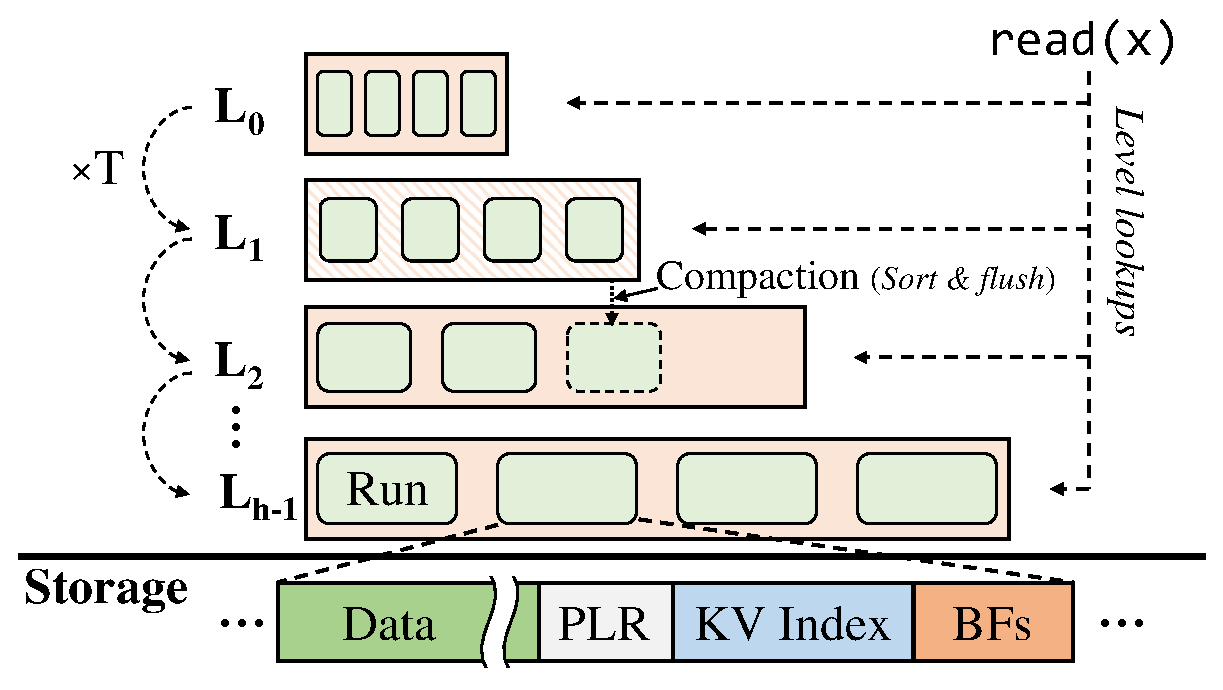
\includegraphics[height=3.3cm]{fig2.eps}
\includegraphics[height=2.4cm]{figs/figs-final/revised/plr-ctr.eps}
\vspace{-10pt}
\caption{FPR control in PLR}
\vspace{-10pt}
\label{fig:plr-control}
\end{figure}

\end{comment}




